% Verbatim from minor_report/chapters/chapter_4_results.tex lines 1115-1326 (retired report),
% headings demoted by 1 level(s). Do not edit here; edit the source of the numbers.

\begin{queried}[Excluded: dynamic-scene trajectory results]
Every dynamic-scene trajectory result in this section, and the anomalies A3 and
A4 that derive from them, are \textbf{withheld as findings} and retained only as
excluded evidence. The reason is the environment, not the measurement: the
dynamic worlds move their props along scripted kinematic paths. The props carry
collision geometry but produce no dynamic response against the robot, nothing
constrains their speeds or routes to warehouse traffic, and they can occupy the
same space as the vehicle without consequence. Numbers measured there describe
the simulation, not the problem the thesis poses.

The runs happened, the artifacts are intact, and the plausibility failures are
real properties of those recordings, so they are reported below rather than
deleted --- an excluded measurement that explains a methodological correction is
worth more in the record than a gap. What must not be done is to read them as
evidence about estimator behaviour in a dynamic warehouse.

Two consequences follow. The condition this work is named for currently has no
valid testbed: it is untested, not tested and failed. And the environment becomes
the leading candidate explanation for the breakdown itself, displacing the
open question left in \cref{sec:anomaly-catalogue} --- testable by rebuilding the
worlds with physically simulated props and re-running, which requires no change
to either estimator.

Unaffected: the static-scene results here, the estimator comparison of
\cref{sec:results-proprio}, the detector evaluation of
\cref{sec:yolo-performance} --- prop motion is kinematic, which changes contact
physics rather than appearance, so detectability and class assignment are
untouched --- and the map evaluation of \cref{sec:map-quality}.
\end{queried}

Table~\ref{tab:trajectory-errors} reports medians and IQRs because the dynamic-run
distributions are strongly skewed. In static scenes, VINS attained a median
translational ATE RMSE of \SI{0.370}{\metre} and rotational RMSE of
\SI{1.56}{\degree} over nine valid runs. The nine valid static ORB runs attained
\SI{0.454}{\metre} and \SI{17.92}{\degree}. The orientation difference is much
larger than the positional difference and must be retained as a separate result.
\Cref{sec:rpe} shows that it is produced almost entirely by one or two discrete
events per run rather than by continuously worse orientation tracking.

\begin{table}[htbp]
\centering
\caption[Trajectory error against rosbag ground truth, median (IQR).]{Trajectory error against rosbag ground truth, median (IQR). ``Clean'' is
ATE RMSE after independently aligning the longest segment without an implied
speed above \SI{10}{\metre\per\second}. Requested VINS+YOLO values are not
active-filter measurements.}
\label{tab:trajectory-errors}
\resizebox{\textwidth}{!}{%
\begin{tabular}{llrrrr}
\toprule
Scene & Requested mode & ATE RMSE (m) & Rotation RMSE (deg) & Clean ATE (m) & Jumps \\
\midrule
Static & VINS-Fusion & $0.370\;(0.063)$ & $1.56\;(0.98)$ & $0.370\;(0.063)$ & $0\;(0)$ \\
Static & ORB-SLAM3 & $0.454\;(0.157)$ & $17.92\;(1.72)$ & $0.341\;(0.151)$ & $1\;(1)$ \\
Dynamic & VINS-Fusion & $724.13\;(823.52)$ & $53.97\;(39.38)$ & $6.80\;(2.57)$ & $1116\;(1157.75)$ \\
Dynamic & ORB-SLAM3 & $190.48\;(2315.44)$ & $108.29\;(116.13)$ & $1.42\;(0.89)$ & $484\;(418.5)$ \\
Dynamic & VINS-Fusion+YOLO$^{*}$ & $738.63\;(1251.84)$ & $56.50\;(37.88)$ & $5.91\;(5.53)$ & $1559.5\;(717)$ \\
Dynamic & ORB-SLAM3+YOLO & $556.05\;(769.39)$ & $138.42\;(60.34)$ & $1.06\;(1.58)$ & $208\;(225.5)$ \\
\bottomrule
\multicolumn{6}{l}{$^{*}$Filter requested but no detection frame was matched.}
\end{tabular}}
\end{table}

Every dynamic run contains at least one impossible-speed step. Nine of 12
baseline VINS runs, all 12 baseline ORB runs, 10 of 12 nominal VINS+YOLO runs,
and all 12 ORB+YOLO runs also exceeded the reference-free mean-speed limit of
\SI{3}{\metre\per\second}. Peak translational error exceeded \SI{50}{\metre} in
9, 12, 10, and 10 runs respectively. Global ATE is therefore dominated by
trajectory breakdown. The clean-segment ATE is substantially smaller, which an
earlier draft read as evidence that the runs contain locally coherent intervals.
\Cref{sec:rpe} withdraws that reading: measured directly, the jump-free
relative error is \SIrange{1.8}{3.8}{\metre} per second, so the estimate is
locally wrong by more than the distance the robot travels. Aligning a short
segment absorbs much of that error, which is why clean-segment ATE looked
reassuring.

The per-repeat values behind those aggregates are given in
\cref{tab:truth-summary}.

\subsubsection{Relative pose error}
\label{sec:rpe}

RPE was implemented after the reporting cutoff and applied to the campaign
without re-running any estimator; \cref{sec:method-trajectory} defines it. It is
reported here because it needs no global alignment, so unlike ATE it cannot be
distorted by a single discontinuity re-seating the rigid fit.
\Cref{tab:rpe-summary} gives the headline interval.

\begin{table}[htbp]
\centering
\caption[Relative pose error at $\Delta=\SI{1}{\second}$, median (IQR) over runs.]{Relative pose error at $\Delta=\SI{1}{\second}$, median (IQR) over runs.
``Jump-free'' excludes pairs spanning a detected tracking jump; the difference
between the two columns is the teleport contribution. Requested VINS+YOLO values
are not active-filter measurements.}
\label{tab:rpe-summary}
\footnotesize
\setlength{\tabcolsep}{3pt}
% Generated by script/make_result_tables.py from
% output/compare/relogged_20260916/trajectory_metrics.csv.
% Do not edit by hand; regenerate instead.
\begin{tabular}{llrrrrr}
\toprule
& & & \multicolumn{2}{c}{Translational (m)} & \multicolumn{2}{c}{Rotational (deg)} \\
\cmidrule(lr){4-5}\cmidrule(lr){6-7}
Scene & Requested mode & Jumps & all pairs & jump-free & all pairs & jump-free \\
\midrule
Static & VINS-Fusion & 0\,(0) & 0.063\,(0.027) & 0.063\,(0.027) & 0.57\,(0.05) & 0.57\,(0.05) \\
Static & ORB-SLAM3 & 1\,(1) & 0.310\,(0.308) & 0.096\,(0.064) & 10.56\,(0.69) & 0.25\,(0.33) \\
\midrule
Dynamic & VINS-Fusion & 1116\,(1158) & 44.652\,(49.397) & 2.825\,(1.595) & 2.05\,(1.63) & 2.76\,(2.01) \\
Dynamic & ORB-SLAM3 & 484\,(418) & 19.477\,(158.567) & 2.079\,(0.267) & 15.15\,(4.82) & 2.49\,(2.51) \\
Dynamic & VINS-Fusion+YOLO$^{*}$ & 1560\,(717) & 44.106\,(95.564) & 3.784\,(1.611) & 2.33\,(4.76) & 2.72\,(1.02) \\
Dynamic & ORB-SLAM3+YOLO & 208\,(226) & 38.174\,(78.432) & 1.805\,(0.634) & 21.60\,(9.72) & 6.33\,(10.39) \\
\bottomrule
\end{tabular}

\end{table}

Two results follow, and the first corrects this chapter.

\paragraph{The dynamic runs are not locally coherent.} Excluding every pair that
spans a jump, dynamic translational RPE at $\Delta=\SI{1}{\second}$ is still
\SIrange{1.8}{3.8}{\metre}. The robot covers about \SI{1.4}{\metre} in that
second, so between teleports the estimate misstates its own motion by more than
the distance travelled. Against the static runs, whose jump-free figures are
\SIrange{0.063}{0.096}{\metre}, dynamic local error is \num{20} to \num{60}
times worse. The corruption is therefore continuous, not confined to isolated
steps, and the earlier reading of clean-segment ATE as evidence of local
coherence does not survive. This was a registered prediction before the metric
was run, and it failed in the direction that matters.

\begin{table}[htbp]
\centering
\caption[Jump-free translational RPE against interval, median over runs, in metres.]{Jump-free translational RPE against interval, median over runs, in
metres. ``Growth'' is the ratio from \SI{0.5}{\second} to \SI{5}{\second};
linear accumulation would give \num{10}$\times$ and a pure random walk
\num{3.2}$\times$.}
\label{tab:rpe-sweep}
\small
\setlength{\tabcolsep}{5pt}
% Generated by script/make_result_tables.py from
% output/compare/relogged_20260916/trajectory_metrics.csv.
% Do not edit by hand; regenerate instead.
\begin{tabular}{llrrrrr}
\toprule
Scene & Requested mode & \SI{0.5}{\second} & \SI{1.0}{\second} & \SI{2.0}{\second} & \SI{5.0}{\second} & Growth \\
\midrule
Static & VINS-Fusion & 0.038 & 0.063 & 0.112 & 0.252 & 6.7$\times$ \\
Static & ORB-SLAM3 & 0.057 & 0.096 & 0.162 & 0.307 & 5.4$\times$ \\
\midrule
Dynamic & VINS-Fusion & 1.524 & 2.825 & 5.067 & 10.082 & 6.6$\times$ \\
Dynamic & ORB-SLAM3 & 1.158 & 2.079 & 3.776 & 6.787 & 5.9$\times$ \\
Dynamic & VINS-Fusion+YOLO$^{*}$ & 2.189 & 3.784 & 5.455 & 10.985 & 5.0$\times$ \\
Dynamic & ORB-SLAM3+YOLO & 0.976 & 1.805 & 3.041 & 4.384 & 4.5$\times$ \\
\bottomrule
\end{tabular}

\end{table}

\Cref{tab:rpe-sweep} shows why this is one mechanism rather than two. Error grows
with interval at \numrange{4.5}{6.7}$\times$ over a tenfold increase in
$\Delta$, and that growth exponent is the same for static and dynamic scenes;
only the magnitude differs, by roughly \num{40}$\times$. The dynamic runs are
not failing in a qualitatively different way from the static ones --- they are
running the same error process far hotter.

\paragraph{ORB-SLAM3's static rotational penalty is entirely jump-localised.}
Static ORB-SLAM3 carries a rotational ATE of \SI{17.92}{\degree} against
VINS-Fusion's \SI{1.56}{\degree}, an elevenfold gap that invites the reading
that ORB-SLAM3 tracks orientation poorly. RPE refutes it. Across the nine static
ORB runs, all-pairs rotational RPE is \SIrange{9.28}{11.63}{\degree}, but
jump-free rotational RPE is \SIrange{0.10}{0.66}{\degree} --- at or below
VINS-Fusion's \SIrange{0.49}{0.69}{\degree} on the same recordings. Every one of
those runs contains one or two jumps and no more.

The whole rotational gap is thus produced by one or two discrete re-seating
events per run, not by continuously worse tracking. This gives anomaly~A5 its
significance: that jump occurs near \SI{2.6}{\second}, immediately before
inertial initialization completes, and it is predominantly rotational. Between
those events ORB-SLAM3's orientation tracking is competitive with VINS-Fusion's.
No causal mechanism is established here --- the association is temporal --- but
the error is now localized to an event rather than attributed to the estimator's
steady-state behaviour.

\begin{sidewaystable}[p]
\centering
\caption[Truth-based trajectory error for every repeat of the relogged campaign.]{Truth-based trajectory error for every repeat of the relogged
campaign. Every dataset is a no-floor-texture world, so that shared part of each
dataset name is omitted. ``ATE'' and ``clean'' are global and
longest-clean-segment ATE RMSE in metres, ``rot'' is rotational geodesic RMSE in
degrees, and ``jmp'' counts steps implying more than \SI{10}{\metre\per\second}.
All 66 runs are operational; two static ORB run summaries have incomplete
schemas, and only one of 12 ORB baseline/filter pairs passed input matching.
Static datasets were not run in either filtered mode; those cells are set to --.}
\label{tab:truth-summary}
\scriptsize
\setlength{\tabcolsep}{4pt}
% Generated by script/make_result_tables.py from
% output/compare/relogged_20260916/trajectory_metrics.csv.
% Do not edit by hand; regenerate instead.
\begin{tabular}{llrrrrrrrrrrrrrrrr}
\toprule
& & \multicolumn{4}{c}{VINS-Fusion} & \multicolumn{4}{c}{ORB-SLAM3} & \multicolumn{4}{c}{VINS-Fusion+YOLO$^{*}$} & \multicolumn{4}{c}{ORB-SLAM3+YOLO} \\
\cmidrule(lr){3-6}\cmidrule(lr){7-10}\cmidrule(lr){11-14}\cmidrule(lr){15-18}
Dataset & Rep & ATE & rot & clean & jmp & ATE & rot & clean & jmp & ATE & rot & clean & jmp & ATE & rot & clean & jmp \\
& & (m) & (deg) & (m) & (n) & (m) & (deg) & (m) & (n) & (m) & (deg) & (m) & (n) & (m) & (deg) & (m) & (n) \\
\midrule
dynamic 00\_000 & 01 & 596.37 & 38.5 & 6.77 & 858 & 45.21 & 176.5 & 1.31 & 109 & 392.55 & 107.0 & 5.74 & 1122 & 13.84 & 76.7 & 1.31 & 37 \\
dynamic 00\_000 & 02 & 206.97 & 92.2 & 8.32 & 609 & 857.95 & 162.0 & 0.84 & 512 & 466.72 & 108.0 & 4.39 & 1183 & 892.31 & 129.9 & 2.45 & 213 \\
dynamic 00\_000 & 03 & 324.01 & 88.4 & 5.47 & 580 & 3364.34 & 70.8 & 1.40 & 610 & 318.66 & 108.7 & 6.07 & 991 & 81.20 & 173.1 & 4.33 & 119 \\
dynamic 00\_001 & 01 & 1030.40 & 63.6 & 2.18 & 1374 & 3002.57 & 29.7 & 1.26 & 1150 & 2309.93 & 74.6 & 2.04 & 1805 & 2885.77 & 82.2 & 1.42 & 1159 \\
dynamic 00\_001 & 02 & 1481.00 & 62.8 & 2.14 & 1695 & 2669.73 & 26.1 & 1.09 & 1141 & 2129.97 & 75.2 & 1.51 & 1810 & 553.35 & 93.5 & 1.98 & 454 \\
dynamic 00\_001 & 03 & 1724.94 & 175.1 & 2.55 & 1995 & 2311.30 & 23.1 & 1.45 & 1098 & 1457.89 & 59.6 & 2.03 & 1997 & 558.76 & 112.8 & 2.82 & 378 \\
dynamic 01\_000 & 01 & 904.94 & 53.3 & 7.29 & 1608 & 98.88 & 169.1 & 4.05 & 239 & 698.15 & 52.0 & 8.67 & 1545 & 8.20 & 102.3 & 0.26 & 44 \\
dynamic 01\_000 & 02 & 851.90 & 53.8 & 7.55 & 1596 & 115.45 & 172.4 & 2.28 & 327 & 796.03 & 52.6 & 7.77 & 1582 & 14.78 & 173.8 & 0.41 & 26 \\
dynamic 01\_000 & 03 & 965.82 & 54.1 & 7.14 & 1619 & 107.60 & 167.7 & 0.64 & 456 & 779.10 & 53.3 & 7.79 & 1574 & 749.16 & 162.6 & 0.45 & 203 \\
dynamic 02\_000 & 01 & 12.49 & 6.1 & 6.80 & 72 & 37.83 & 59.3 & 2.09 & 388 & 4518.77 & 25.1 & 2.09 & 2610 & 1097.95 & 159.7 & 0.54 & 231 \\
dynamic 02\_000 & 02 & 12.88 & 5.5 & 7.36 & 61 & 265.50 & 62.9 & 2.17 & 689 & 11.85 & 6.4 & 7.55 & 62 & 737.27 & 148.9 & 0.81 & 219 \\
dynamic 02\_000 & 03 & 11.30 & 4.3 & 6.81 & 58 & 42.37 & 145.8 & 1.72 & 408 & 12.55 & 6.9 & 6.29 & 66 & 15.81 & 146.9 & 0.59 & 31 \\
\midrule
static 000 & 01 & 0.37 & 1.6 & 0.37 & 0 & 0.58 & 17.9 & 0.55 & 1 & -- & -- & -- & -- & -- & -- & -- & -- \\
static 000 & 02 & 0.41 & 1.5 & 0.41 & 0 & 0.79 & 20.4 & 0.77 & 1 & -- & -- & -- & -- & -- & -- & -- & -- \\
static 000 & 03 & 0.43 & 1.6 & 0.43 & 0 & 1.20 & 19.1 & 0.30 & 2 & -- & -- & -- & -- & -- & -- & -- & -- \\
static 001 & 01 & 0.39 & 2.3 & 0.39 & 0 & 0.45 & 18.9 & 0.27 & 2 & -- & -- & -- & -- & -- & -- & -- & -- \\
static 001 & 02 & 0.29 & 1.8 & 0.29 & 0 & 0.45 & 18.1 & 0.21 & 2 & -- & -- & -- & -- & -- & -- & -- & -- \\
static 001 & 03 & 0.48 & 2.2 & 0.48 & 0 & 0.38 & 17.2 & 0.26 & 1 & -- & -- & -- & -- & -- & -- & -- & -- \\
static 002 & 01 & 0.34 & 0.8 & 0.34 & 0 & 0.42 & 16.7 & 0.39 & 1 & -- & -- & -- & -- & -- & -- & -- & -- \\
static 002 & 02 & 0.36 & 0.8 & 0.36 & 0 & 0.46 & 17.6 & 0.43 & 1 & -- & -- & -- & -- & -- & -- & -- & -- \\
static 002 & 03 & 0.34 & 0.7 & 0.34 & 0 & 0.36 & 16.9 & 0.34 & 1 & -- & -- & -- & -- & -- & -- & -- & -- \\
\bottomrule
\end{tabular}


\vspace{1ex}
\raggedright\footnotesize
$^{*}$Filter requested but no detection frame was matched in any repeat; these
columns are not active-filter measurements.
\end{sidewaystable}

\begin{figure}[htbp]
  \centering
  % The summary table belongs with these panels, so it is set inside the float
  % rather than as a separate table that page-breaking could carry away.
  {\small\setlength{\tabcolsep}{3pt}% Generated by script/make_result_tables.py from
% output/compare/relogged_20260916/trajectory_metrics.csv.
% Do not edit by hand; regenerate instead.
\begin{tabular}{lrrrrrrr}
\toprule
Requested mode & Poses & Overlap & Path & ATE RMSE & Rot RMSE & Clean ATE & Jumps \\
& (n) & (s) & (m) & (m) & (deg) & (m) & (n) \\
\midrule
VINS-Fusion & 1494 & 77.0 & 5486.93 & 596.367 & 38.51 & 6.771 & 858 \\
ORB-SLAM3 & 1105 & 77.3 & 408.22 & 45.206 & 176.53 & 1.314 & 109 \\
VINS-Fusion+YOLO$^{*}$ & 2175 & 77.1 & 1958.14 & 392.546 & 107.04 & 5.743 & 1122 \\
ORB-SLAM3+YOLO & 943 & 77.2 & 239.53 & 13.839 & 76.72 & 1.310 & 37 \\
\bottomrule
\end{tabular}
}

  \vspace{0.5ex}
  {\footnotesize $^{*}$Filter requested but no detection frame was matched.}

  \vspace{2ex}
  % The image carries its own rendered title, the same summary table, and a
  % footnote in the top 310 px of 2496; that band is trimmed away because those
  % numbers are now typeset above.
  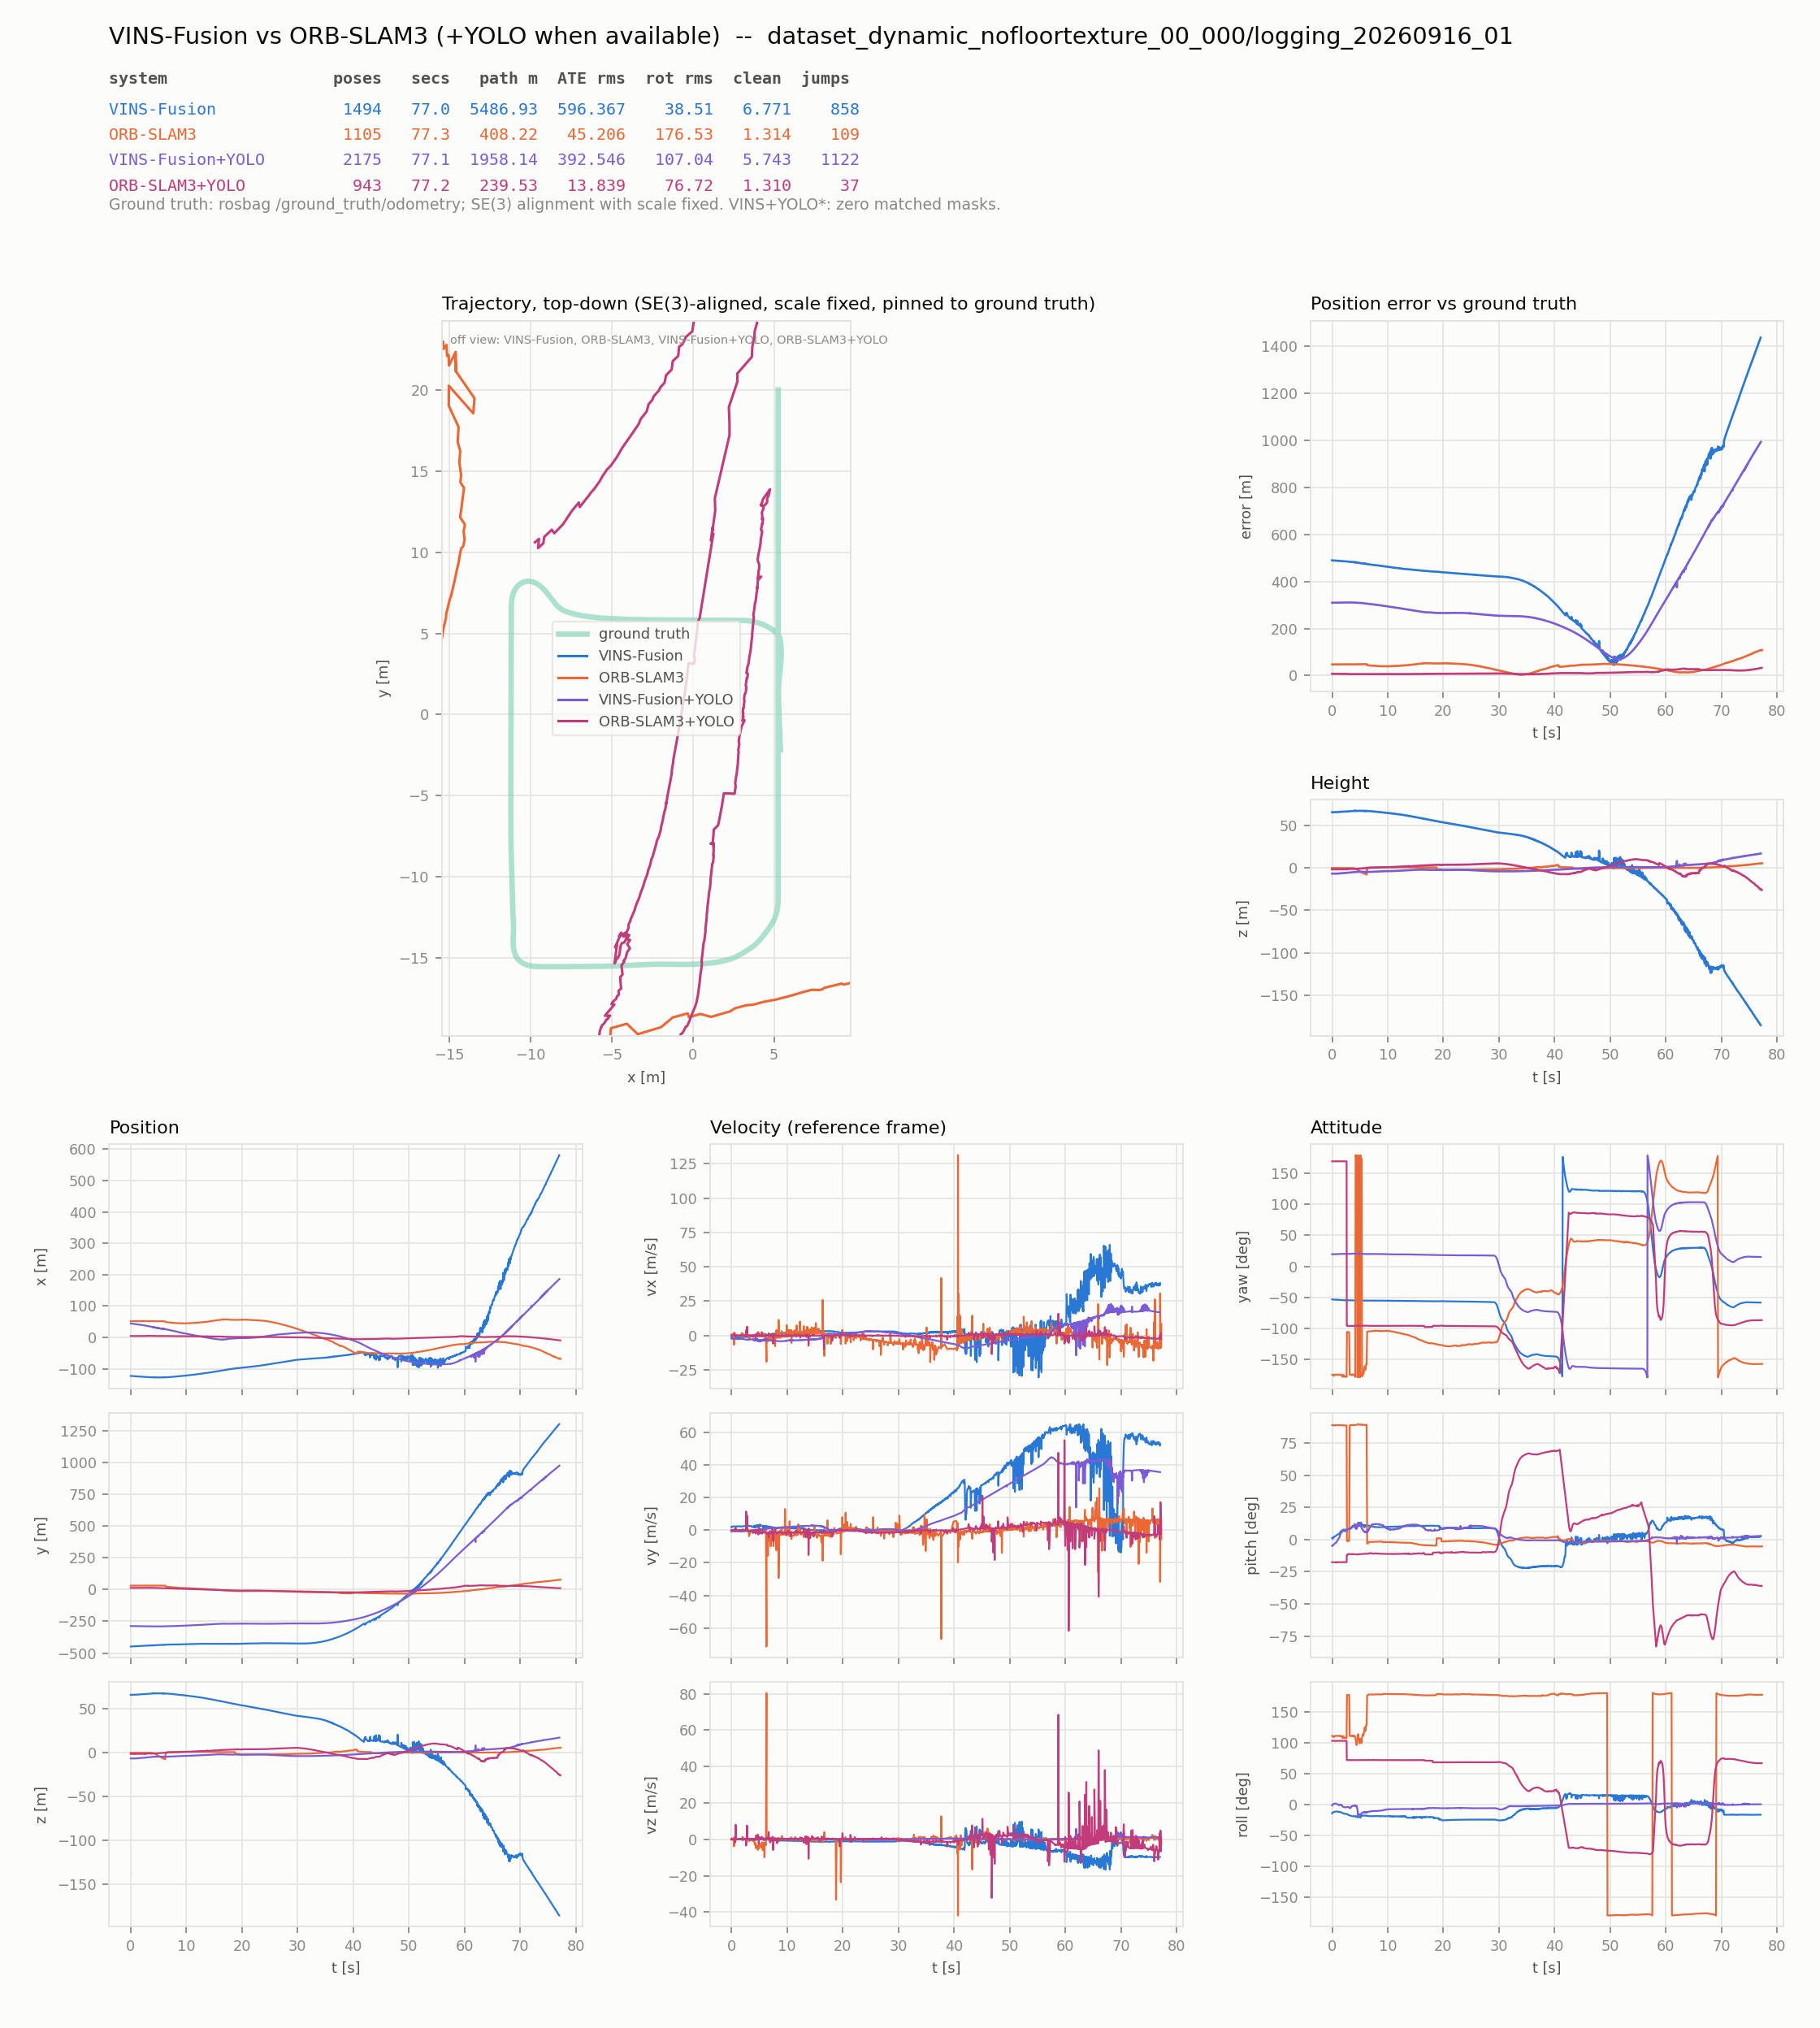
\includegraphics[width=\textwidth, trim={0 0 0 140pt}, clip]{../../../output/compare/relogged_20260916/simulation/dataset_dynamic_nofloortexture_00_000/logging_20260916_01/compare_light.png}
  \caption[Representative repeated-run trajectory diagnostic for \repo{dataset_dynamic_nofloortexture_00_000/logging_20260916_01}, in the same visual format as the existing comparison figures.]{Representative repeated-run trajectory diagnostic for
  \repo{dataset_dynamic_nofloortexture_00_000/logging_20260916_01}, in the same
  visual format as the existing comparison figures. The table gives the
  per-system summary for this run; ``clean'' is ATE RMSE over the longest
  jump-free segment. The very large paths and frequent jumps are retained rather
  than clipped into a favourable view. ATE and rotational errors use the rosbag
  \repo{/ground_truth/odometry} topic after rigid $SE(3)$ alignment with scale
  fixed. The nominal VINS+YOLO trace is invalid as a filtering treatment because
  no masks were matched.}
  \label{fig:relogged-trajectory-example}
\end{figure}

Baseline ORB-SLAM3 logged $7.75\pm6.03$ tracking-loss events and
$9.52\pm6.49$~s of lost tracking per dynamic run (mean $\pm$ sample SD,
$n=12$). ORB+YOLO logged $9.17\pm3.01$ events and $11.46\pm5.32$~s. VINS logged
no estimator resets in either requested mode, but the absence of resets does not
make its trajectories plausible. The event types are estimator-specific and are
not treated as numerically equivalent.

\begin{figure}[htbp]
  \centering
  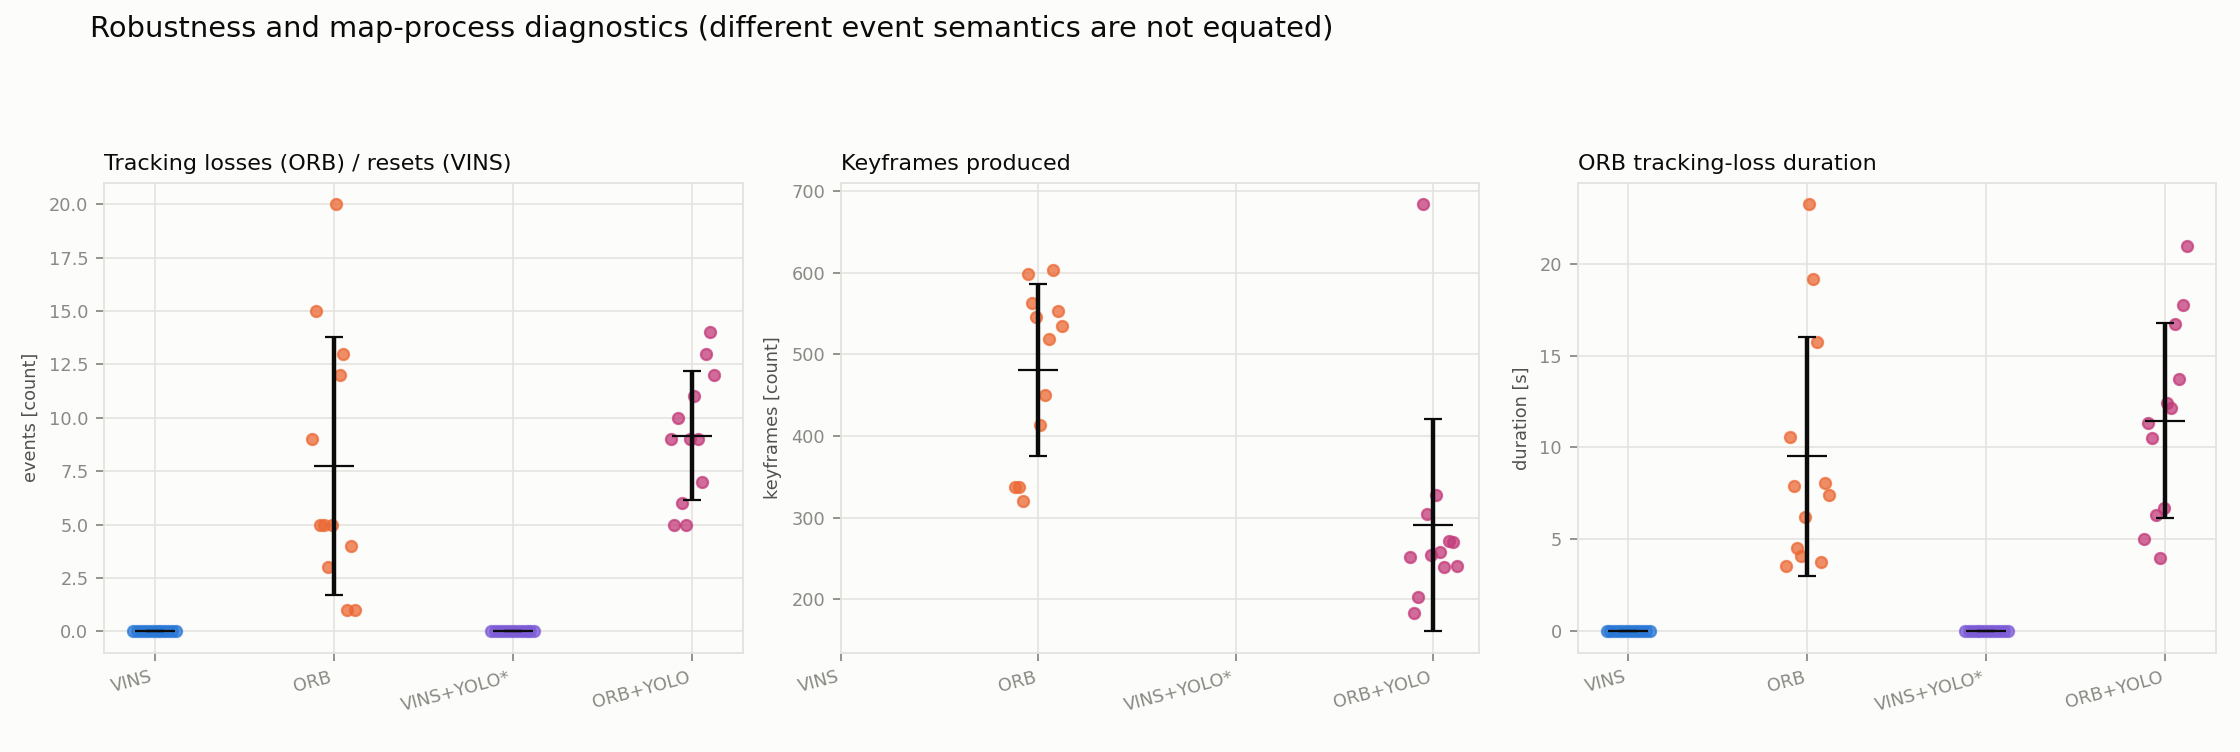
\includegraphics[width=\textwidth]{../../../output/compare/relogged_20260916/robustness_light.png}
  \caption[Per-run robustness and keyframe observations for the dynamic datasets.]{Per-run robustness and keyframe observations for the dynamic datasets.
  Points are experimental runs and black marks are mean $\pm$ sample SD. VINS
  reset count and ORB tracking-loss count have different semantics. The asterisk
  identifies the requested VINS filter mode in which no masks were matched.}
  \label{fig:robustness-results}
\end{figure}
